In this chapter, I will describe the implementation of the website generator.
I will start by discussing the choice of technology, followed by the project settings.
Then, I will describe the code structure, user interface, and functionality.
Finally, I will discuss the licensing of the libraries used in the project.


\section{Choosing the Technology}
The main factor in choosing the technology is the ability to generate a website that can be easily deployed and accessed by users.
In the design chapter, I concluded that I would use a common format with all gRPC definitions, and the website would be generated from this format in the browser.
Therefore, I must choose a technology for the website and the common format generators.

As for the website, the basics are done using HTML and CSS\@.
There is no other choice.
For the programming language, because of the dynamic rendering based on the common format, the only possibilities are JavaScript and WebAssembly.
Because I will need to be updating the website (meaning the DOM), which is not supported directly by WebAssembly, I have chosen JavaScript~\cite{webassembly-dom}.

JavaScript was initially designed to manage basic website interactions using simple scripts.
The website will not be a simple script though, but many scripts with complex functions and classes.
Complexity can lead to subtle bugs that are hard to track down in plain JavaScript.
Adding type-checking ensures that errors are caught at the development stage, reducing bugs and improving code quality.
Additionally, type annotations make the code more readable and easier to understand, which is crucial when collaborating with others or for future modifications.
\cite{typescript-why-create}

Based on the State of JavaScript 2022 survey~\cite{state-of-js-other-tools}, the most popular language flavor of JavaScript is Typescript\footnote{\url{https://www.typescriptlang.org/}}.
Because of the popularity, the benefits of type-checking, and the readability of the code, I have decided to use TypeScript for the website.

The browser does not limit the common format generator language selection because the generators are run on the developer's machine.
Therefore, the language choice is based on the required libraries for the generators.
But, because I will be using the protobufjs JavaScript library, I will use JavaScript for the generators.

\subsection{Web Framework}
To create the website with extensive logic, I will use a front-end framework.
The most popular options for the web framework based on the State of Javascript 2022 survey are React\footnote{\url{https://react.dev/}}, Angular\footnote{\url{https://angular.io/}}, Vue.js\footnote{\url{https://vuejs.org/}}, and Svelte\footnote{\url{https://svelte.dev/}}~\cite{state-of-js-frontend-frameworks}.
I want the page to exist for a long time and be maintained.
For this reason, I will choose the most popular framework, which is React.

React is a JavaScript library for building user interfaces.
It is maintained by Meta and a community of individual developers and companies.
React can be used as a base in the development of single-page web applications.
It allows developers to create large web applications that can change data without reloading the page, making the website faster.
\cite{react}

Using React is a great option, but it requires a lot of manual setup (routing, code splitting, and more).
For this reason, there is a React framework called Next.js\footnote{\url{https://nextjs.org/}}.
It simplifies the setup, development, static site page generation, routing, and a lot more~\cite{nextjs}.
It is also the first recommended way to build a new React application by the React team~\cite{react-start-new-project}.
Therefore, I will use Next.js for the website.
The key features, except the setup of Next.js, that I will use are static site generation and TypeScript support.

\subsection{Styling Libraries}
Instead of using my own CSS classes to style the website, I will use a framework to speed up development.
The most popular CSS frameworks based on the State of CSS 2023 survey are Bootstrap\footnote{\url{https://getbootstrap.com/}}, Tailwind CSS\footnote{\url{https://tailwindcss.com/}}, and Materialize CSS\footnote{\url{https://materializecss.com/}}~\cite{state-of-css-frameworks}.
All of them are good options, but as for choosing the front-end framework, I will choose the most popular one, which is Bootstrap.

\subsection{Protobufjs Library}
Based on the design chapter, the protobufjs library is used to serialize and deserialize the data in a common JSON format.
The library also offers a tool called protobufjs-cli\footnote{\url{https://www.npmjs.com/package/protobufjs-cli}}.
It is a command-line tool that can be used to generate the JSON format from the proto files~\cite{protobufjs-cli}.
It has an issue, though.
It only allows individual proto files as input, not the entire folder, which is in the earlier defined use case~\ref{uc:generate-website-from-proto-files}.
Also, the correct parameters need to be specified in order to get the correct output.
For this reason, I will use the protobufjs-cli, but only as a library.
This will allow me to have potential features in the future, fix the current ones, and seal the required parameters.

There are two more issues with this library that need to be addressed.
The first one is that there is a bug in the library when parsing the value options for enums.
I found the issue in the library's repository source code and fixed it locally using the package manager patch functionality.
I have also reported the issue to the library's repository at \url{https://github.com/protobufjs/protobuf.js/issues/1961} with a way to fix it and created a pull request.
The patch change is in the code snippet~\ref{lst:protobufjs-enum-value-options}.

\newpage

\begin{lstlisting}[style=JavaScript, caption={protobufjs library enum comments bug fix}, label={lst:protobufjs-enum-value-options}]
Enum.fromJSON = function fromJSON(name, json) {
    // This line is removed
    var enm = new Enum(name, json.values, json.options, json.comment, json.comments);
    // This line is added
    var enm = new Enum(name, json.values, json.options, json.comment, json.comments, json.valuesOptions);
    enm.reserved = json.reserved;
    return enm;
};
\end{lstlisting}

The second issue is that the protobufjs-cli library does not support comments.
I have found an already existing issue (\url{https://github.com/protobufjs/protobuf.js/issues/1145}), which hints at how to patch the library locally until it is added to the library itself.
To make the protobufjs-cli library support comments, I have slightly updated how JSON exports work and created a local patch.
When this feature is added to the library, I can remove the patch and use the library as it is.
The patch change is in the code snippet~\ref{lst:protobufjs-comments}.

\begin{lstlisting}[style=JavaScript, caption={protobufjs-cli comments support}, label={lst:protobufjs-comments}]
function json_target(root, options, callback) {
    // This line is removed
    callback(null, JSON.stringify(root, null, 2));
    // Theis line is added
    callback(null, JSON.stringify(root.toJSON({ keepComments: true }), null, 2));
}
\end{lstlisting}

\subsection{gRPC-Web Client Library}\label{subsec:grpc-web-client}
% Talk about extracting the gRPC-Web client from the generated stubs
The gRPC-Web library only offers client-side code generation from the proto files (stubs).
However, it does not allow the client to make the requests only with the possibility of implementing the data serialization and deserialization.
I have tried to find a library offering this functionality, but I have not found any.
For this reason, I have decided to analyze how the stubs are generated in order to extract the gRPC-Web client.
I already know that I can serialize and deserialize the data using the protobufjs library, which I will use for that.

There are two generated gRPC-Web client files.
One generates the client, and the other generates the message types and methods.
Note that the client is still specific to the proto files.

Based on the generated code, I have found that the actual call is done using initialization of \textit{GrpcWebClientBase} and then calling \textit{rpcCall} method for unary requests and \textit{serverStreaming} method for server streaming requests.
The client initialization does not require any parameters but can be supplied with the option object, which may contain a format (binary or text).
The \textit{rpcCall} method requires a method name, a request message type object, a metadata of the request, a methodDescriptor (more on that later), and a callback.
The \textit{rpcCall} function returns a stream, which may be used for additional headers or trailer handling.
The \textit{serverStreaming} method requires the same parameters, but the callback is not present, and responses are handled only using the returned stream.

The code snippet~\ref{lst:grpc-web-client} shows an example of the method with parameters.
The method name is a string with a full path to the method.
The request message type is defined by the generated client and is required to contain specific attributes and methods.
Because I am using the protobufjs library, I have found out I am able to supply only an empty object (\textit{\{\}}) there and do the rest of the work in other functions supplied in the method descriptor.

The method descriptor is an object containing the method name, the method type, the request message type, the response message type, and the request serialize and response deserialize functions.
The method name is just the method name without a path.
The method type is either unary or server streaming.
Because I am using the protobufjs library, a fake class with a constructor can replace the request and response message types.
Finally, the request serialize, and response deserialize functions are functions that take the message object and return the serialized or deserialized message.
Because I have replaced the request object with an empty object, the request serialize function is not supplied with the message.
However, I can directly access the variable from the outer scope using the protobufjs library and return the encoded message.
For the response deserialize function, I can use the protobufjs library again to decode the available message, this time as a byte's array parameter, and return it.
The callback function or the stream receives the deserialized message in the protobufjs format.

\begin{lstlisting}[style=JavaScript, caption={gRPC-Web extracted client unary call example}, label={lst:grpc-web-client}]
const client = new GrpcWebClientBase({ format: options?.format });

const unaryStream = client.rpcCall(
    methodPath,
    // Ignored, using protobufjs directly
    {},
    options?.metadata ?? {},
    new MethodDescriptor(
        method.name,
        MethodType.UNARY,
        // Ignored, using protobufjs directly
        DummyRPCType,
        // Ignored, using protobufjs directly
        DummyRPCType,
        () => {
            return typeEncode.encode(message).finish();
        },
        (bytes: Uint8Array) => {
            return typeDecode.decode(bytes);
        },
    ),
    (err, response: protobuf.Message<MessageData>) => {
        if (err) {
            reject(err);
        } else {
            completeResponse.data = [response];
        }
    },
);
\end{lstlisting}


I have extracted the gRPC-Web client from the generated stubs, and I can use it on the website for any request.
The gRPC-Web library still handles the communication with the server, though, so any future updates to the library should be automatically applied to the client as well.

\subsection{Other Libraries}
Other essential libraries that I will use are react-hook-form\footnote{\url{https://react-hook-form.com/}} for creating the request input form validation, yup\footnote{\url{https://github.com/jquense/yup}} for the schema validation (used in connection with forms), and fontawesome\footnote{\url{https://fontawesome.com/}} for the icons.
These libraries have the features I need from them, have over a million weekly downloads (which is significant compared to other NPM packages), and are maintained.
Again, I am choosing the most popular and maintained libraries for the long-term existence of the static documentation website.


\section{Project Settings}
The project is using the Lerna\footnote{\url{https://lerna.js.org/}} and pNpM\footnote{\url{https://pnpm.io/}} package manager.
Lerna is a tool that optimizes the workflow around managing multi-package repositories~\cite{lerna}.
And pNpM is a fast, disk-space efficient package manager with the support of workspaces and libraries patching~\cite{pnpm}.
Both tools cooperate and are compatible with each other.

The project is set up as a monorepo.
It is divided into three packages:
\begin{itemize}
    \item \textbf{proto-to-json} -- contains the generator from proto files,
    \item \textbf{reflection-to-json} -- contains the generator from the reflection file,
    \item \textbf{web} -- contains the website.
\end{itemize}
The project also contains \textit{example} and \textit{patches} folders.

The \textit{example} folder contains example proto and reflection files with a pre-generated common format, as well as Envoy proxy configuration and gRPC server implementation in JavaScript.
The Envoy proxy can then be started using a Docker image \textit{envoyproxy/envoy} and the gRPC server using the \textit{node server.js} command.
This setup can be used to test the website's functionality.

The \textit{patches} folder contains the patches for the protobufjs library described in the~\ref{subsec:grpc-web-client}.
They are split into two files, each containing the diff of a concrete package file.
These files are generated using the \textit{pnpm patch \textless{}pkg name\textgreater{}} command and applied automatically when the package is installed.

The generators from proto and reflection files are set up as NPM runnable packages.
This means the packages can be installed globally and run from the command line.

The website is set up as a Next.js project using the command \textit{npx create-next-app@latest}.
It uses an App directory for routing, TypeScript as the language, ESLint\footnote{\url{https://eslint.org/}} for linting, Jest\footnote{\url{https://jestjs.io/}} for testing, and Prettier\footnote{\url{https://prettier.io/}} for code formatting.
The website is set up to be statically generated using the \textit{output: "export"} option, which means that the website is generated at build time and served as static files.
For building, it uses the Next.js Compiler, which is run using the \textit{pnpm build} command.


\section{JSON from Proto Files Generator}
The generator from proto files is a command-line tool that generates the common JSON format.
It takes one or more proto files or a directory with proto files as input and outputs the JSON format to the console.
The script uses the proto files from the command or recursively traverses the directory for all proto files, which are then passed to the protobufjs-cli library with correct arguments and writes output to the console.
The output can be then redirected to a file.

The code snippet~\ref{lst:proto-to-json} shows an example of the command.
The symbol \textit{\textgreater{}} redirects the output to a file.
The \textit{SOURCE\_PROTO\_FILES} can be any number of proto files or folder combinations split by space.
If invalid proto files are passed, an error will be thrown, which is then displayed in the console.

\begin{lstlisting}[caption={proto-to-json command example}, label={lst:proto-to-json}]
gf-proto-to-json ${SOURCE_PROTO_FILES} > ${EXPORTED_NAME}.json
\end{lstlisting}

The generated JSON output can then be used on the website.


\section{JSON from gRPC Reflection Generator}
The generator from the reflection file is a command-line tool that generates the common JSON format.
The script uses the reflection bin file from the command, which is then processed by the protobufjs library and serialized to the JSON format.
The output can be then redirected to a file.

The bin format can be generated using the grpcurl tool.
The example command is shown in the code snippet~\ref{lst:reflection-to-bin}.
The \textit{BIN\_FILE} is the target reflection bin file, and \textit{GRPC\_SERVER} is the gRPC server address.
The \textit{-protoset-out} is used to output the reflection to the file, and the \textit{describe} tells the grpcurl to output the reflection definitions.
Other parameters and features of the grpcurl tool can also be used (e.g., TLS settings, filtering only parts of the reflection interface, etc.).
This is just an example.
Also, there may be other tools for creating the reflection bin file.
There is no limitation on the tool used as long as the bin file is in the correct format.

\begin{lstlisting}[caption={proto-to-json command example}, label={lst:reflection-to-bin}]
grpcurl -protoset-out ${BIN_FILE}.bin -plaintext ${GRPC_SERVER} describe
\end{lstlisting}

The code snippet~\ref{lst:reflection-to-json} shows an example of the command.
The symbol \textit{\textgreater{}} redirects the output to a file.
The \textit{SOURCE\_BIN\_FILE} is the bin file.
If an invalid bin file is passed, an error will be thrown, which will then be displayed in the console.

\begin{lstlisting}[caption={proto-to-json command example}, label={lst:reflection-to-json}]
gf-reflection-to-json ${SOURCE_BIN_FILE} > ${EXPORTED_NAME}.json
\end{lstlisting}

The generated JSON output can then be used on the website.


\section{Static Website}
The website is static and generated using the Next.js framework.
The code structure is divided into:
\begin{itemize}
    \item \textbf{src/app} -- contains the pages of the website,
    \item \textbf{src/components} -- contains the React components,
    \item \textbf{src/contexts} -- contains the React contexts,
    \item \textbf{src/scss} -- contains the global styles of the website,
    \item \textbf{src/services} -- contains the functions with logic for the website,
    \item \textbf{src/types} -- helper types and constant definition,
    \item \textbf{public} -- contains the public files (e.g., images).
\end{itemize}

After the website is built, the output is in the \textit{out} directory.
The directory contains static HTML, CSS, JavaScript files, and all files from the public directory.
It can then be hosted by any web server that supports static file hosting.
It is enough to copy only the contents of the \textit{out} directory to the server.
The default definitions file is in the root of the directory and is called \textit{definitions.json}.
It is shown on the website page by default.
Any other file can replace it with the same structure and name, or it is possible to host the file anywhere and specify the file URL in the \textit{url} query parameter of the website.


\begin{landscape}
    \begin{figure}
        \centering
        \captionsetup{justification=centering}
        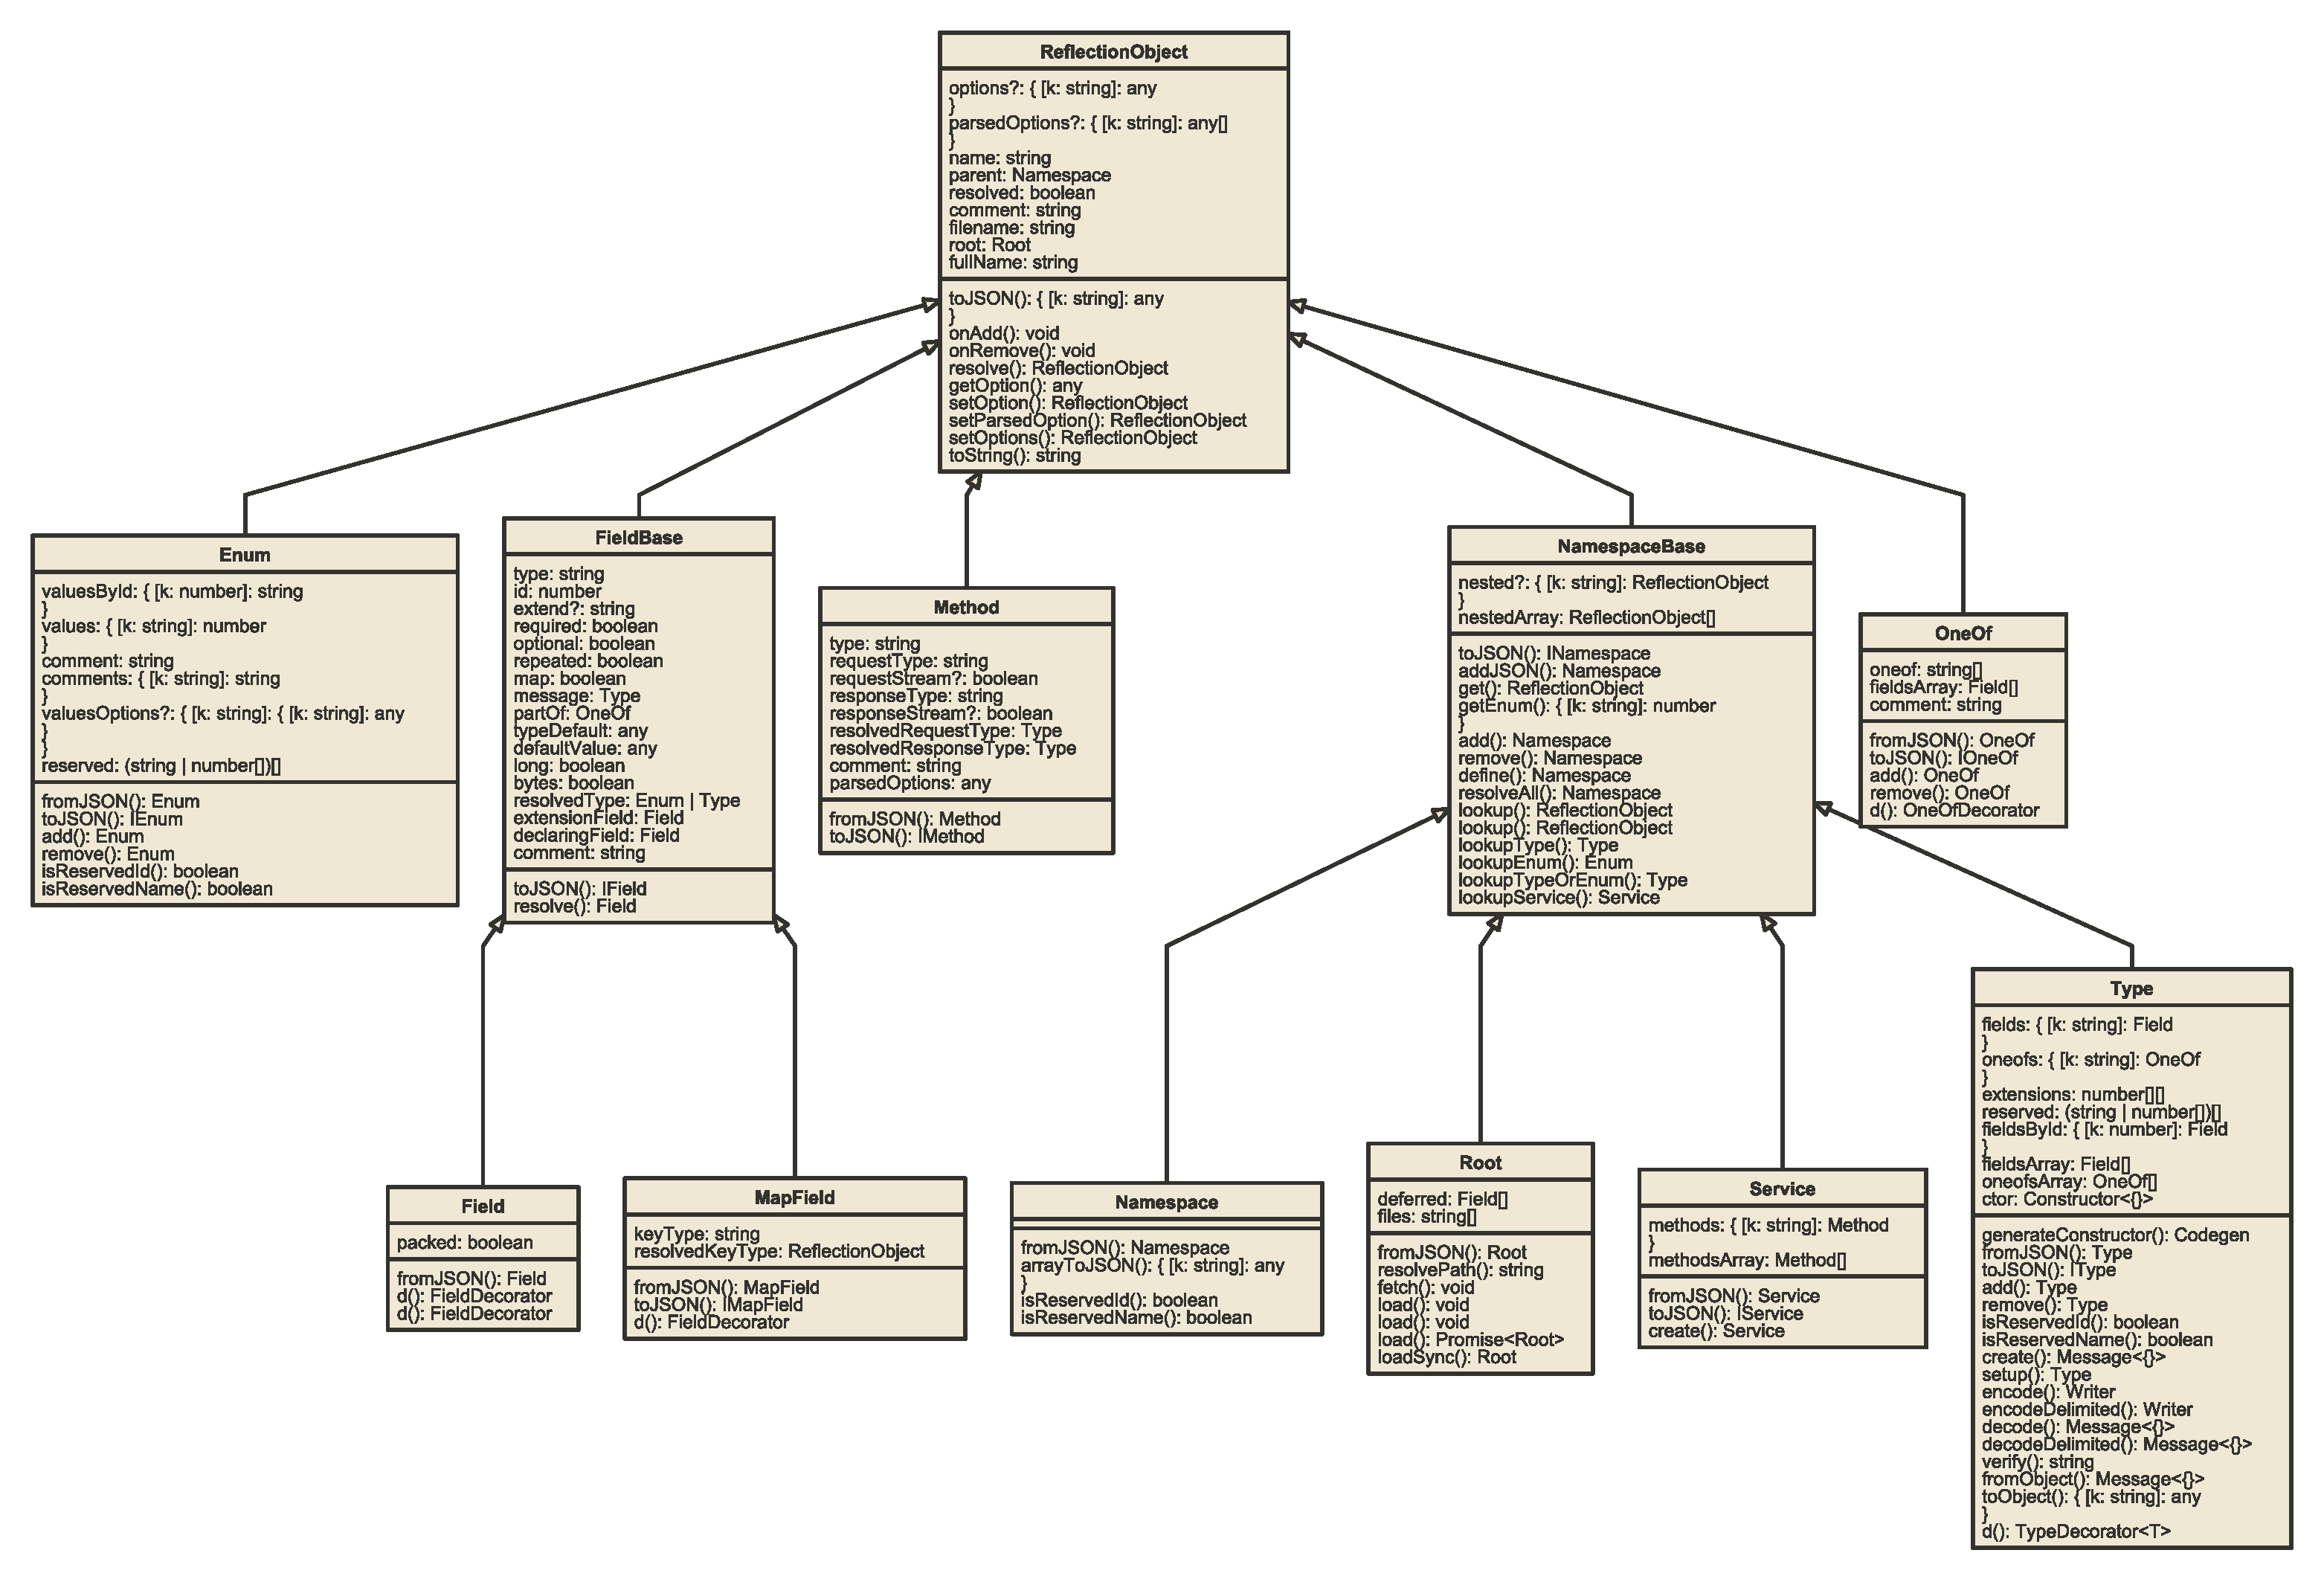
\includegraphics[width=0.75\paperheight]{images/implementation/protobufjs-class-diagram}
        \caption{Protobufjs class diagram~\cite{protobufjs}}
        \label{fig:protobufjs-class-diagram}
    \end{figure}
\end{landscape}

\subsection{Protobufjs Data Structure}
I am using the protobufjs library with its data structure.
The data class diagram is shown in the figure~\ref{fig:protobufjs-class-diagram}.

The base is the \textit{Root} class, which is returned by parsing the common format.
Other classes like service or type create a tree structure.
For example, using the field \textit{nested} (or \textit{nestedArray}) from the \textit{NamespaceBase}, I can traverse the tree and find all services, message types, or enums.
This way, I find all the data I need for the website.

Each class has fields related to the protobuf features.
For example, the \textit{Service} class has a \textit{methods} field containing all methods for that service, and the \textit{Method} class has a field of what type of streaming it is.
Also, all classes have a \textit{comment} field containing the proto file's comment.
Using these fields, I can display the data on the website.

\subsection{Design and Functionality}
The website design starts from the wireframes in the design chapter.
The whole page is in the figure~\ref{fig:implementation-screenshots-fullpage}.
At the top, the toolbar contains the URL input for definitions JSON files by default.
If the user clicks on the URL dropdown button, they can change the input to a file input (shown in the figure~\ref{fig:implementation-screenshots-reflection-input}).
The file can then be a JSON definition file from the local machine or the gRPC reflection bin file.
The file is then parsed, and the data is displayed on the website.

\begin{figure}[!htb]
    \centering
    \captionsetup{justification=centering}
    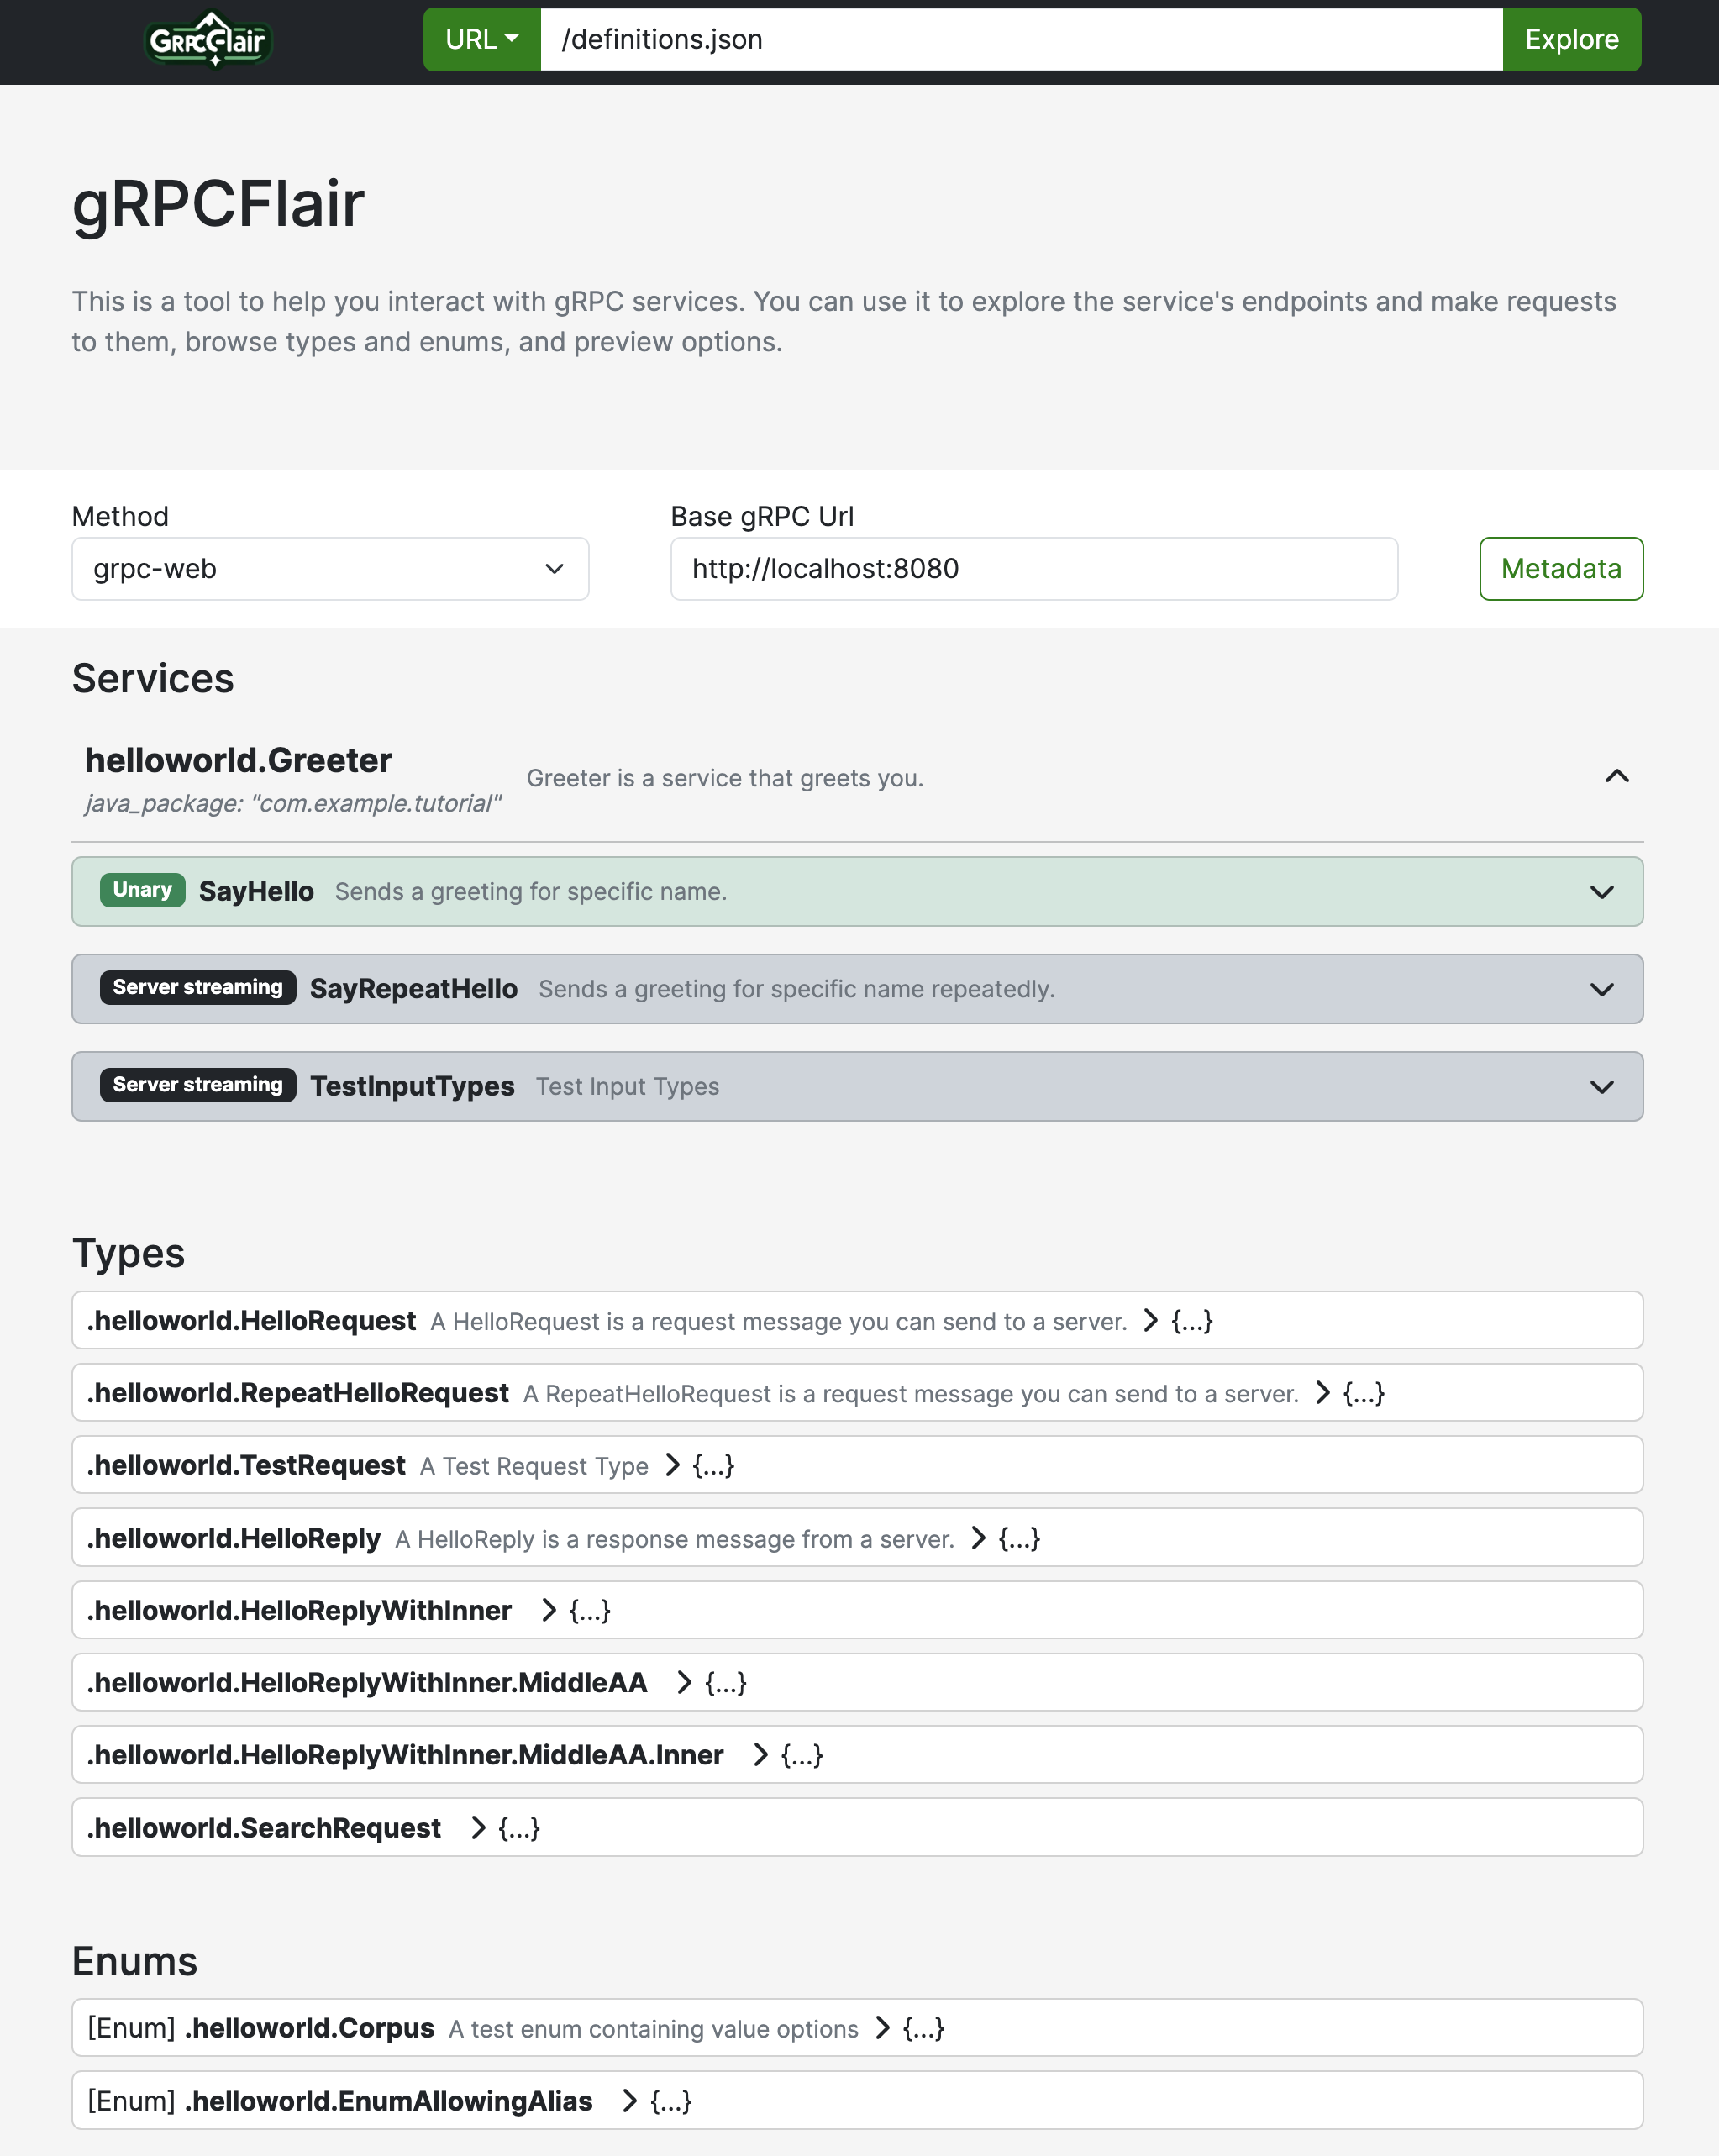
\includegraphics[width=0.8\textwidth]{images/implementation/screenshots/fullpage}
    \caption{Website overview}
    \label{fig:implementation-screenshots-fullpage}
\end{figure}

\begin{figure}[!htb]
    \centering
    \captionsetup{justification=centering}
    
\includegraphics[width=0.8\textwidth]{images/implementation/screenshots/reflection-input}
    \caption{Input using file}
    \label{fig:implementation-screenshots-reflection-input}
\end{figure}

Under the toolbar is a short description of the website's purpose.
Under the description is a section with global settings.
The first is the selection of the backend method, which is, by default, the gRPC-Web.
This is a place where it is possible to add more backends in the future, which may have full implementation of client streaming.
If the gRPC-Web library eventually has client streaming support, this dropdown can be easily removed.

Next to the method selection is a backend gRPC server selection.
The user can change the server address and port.
This is a global setting for the website and is used for all requests.

Next is the global metadata definition.
Upon clicking the button, a modal dialog, figure~\ref{fig:implementation-screenshots-metadata-modal}, is shown.
The user can then define the metadata as key-value pairs for the request.
It also allows defining the authorization token, effectively creating a new metadata entry with a predefined format.

\begin{figure}[!htb]
    \centering
    \captionsetup{justification=centering}
    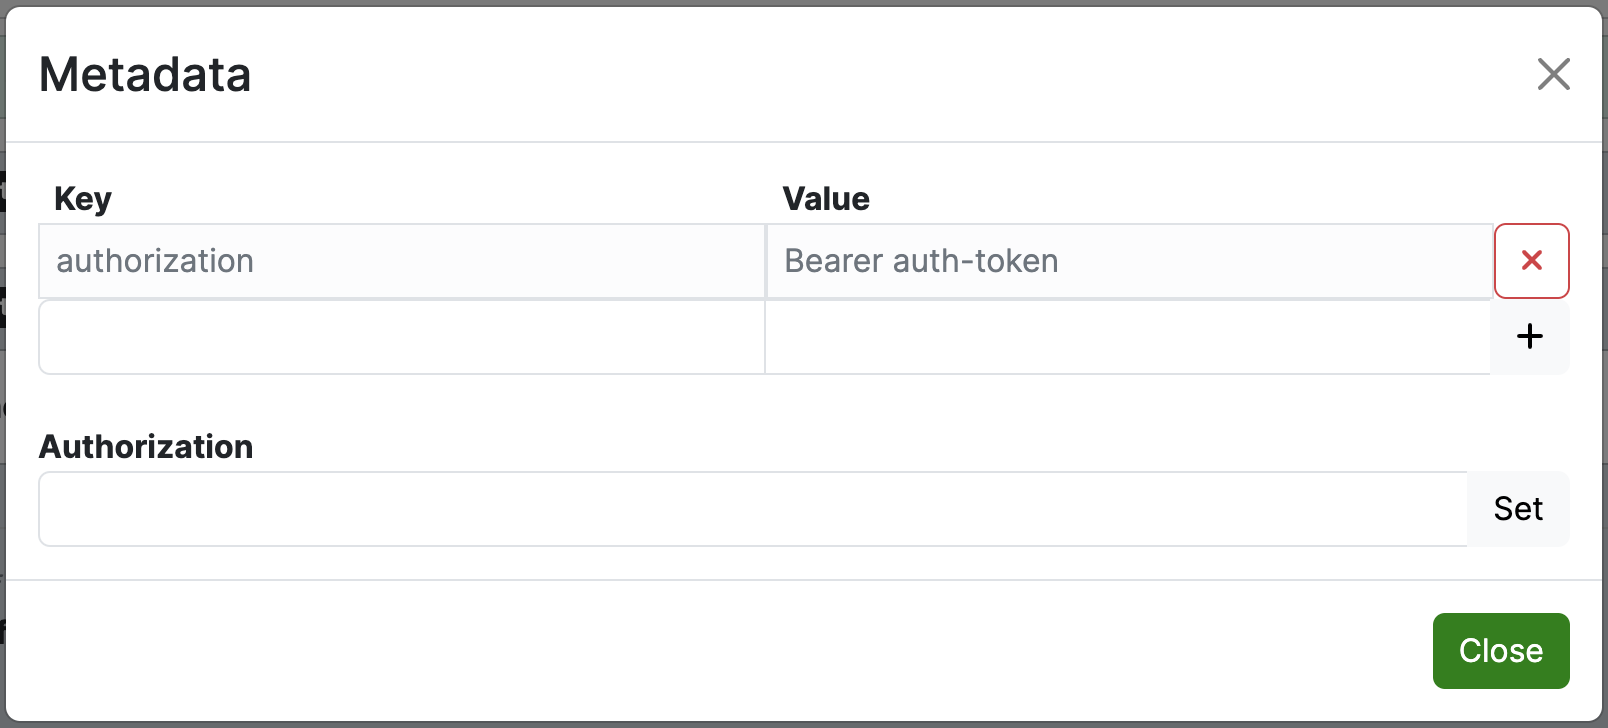
\includegraphics[width=0.7\textwidth]{images/implementation/screenshots/metadata-modal}
    \caption{Metadata modal dialog}
    \label{fig:implementation-screenshots-metadata-modal}
\end{figure}

The list of services is under the global settings.
The services are displayed as described in the design chapter.
In the figure~\ref{fig:implementation-screenshots-fullpage}, the user can also see the difference between the unary and server streaming methods, as well as service options and comments.

The expanded method is shown in the figure~\ref{fig:implementation-screenshots-method}.
Its design is based on the wireframes, where the user can see the request input form and the response message type.
After executing the method, the response is shown as in the figure~\ref{fig:implementation-screenshots-response}.
It contains the request JSON with the metadata, server URL, and the response with headers and trailers.
When the method type is server streaming, the response is shown as in the figure~\ref{fig:implementation-screenshots-responses-streaming} with all responses gradually showing as soon as they arrive.
If the user wants to cancel the method execution while it is still running, they can click the cancel button, which is shown in the figure~\ref{fig:implementation-screenshots-execution-pending}.
If there is an error in the response, it is shown as in the figure~\ref{fig:implementation-screenshots-response-error} with the gRPC error code status, as well as the HTTP status (for gRPC-Web) and metadata.


\begin{figure}[!htb]
    \centering
    \captionsetup{justification=centering}
    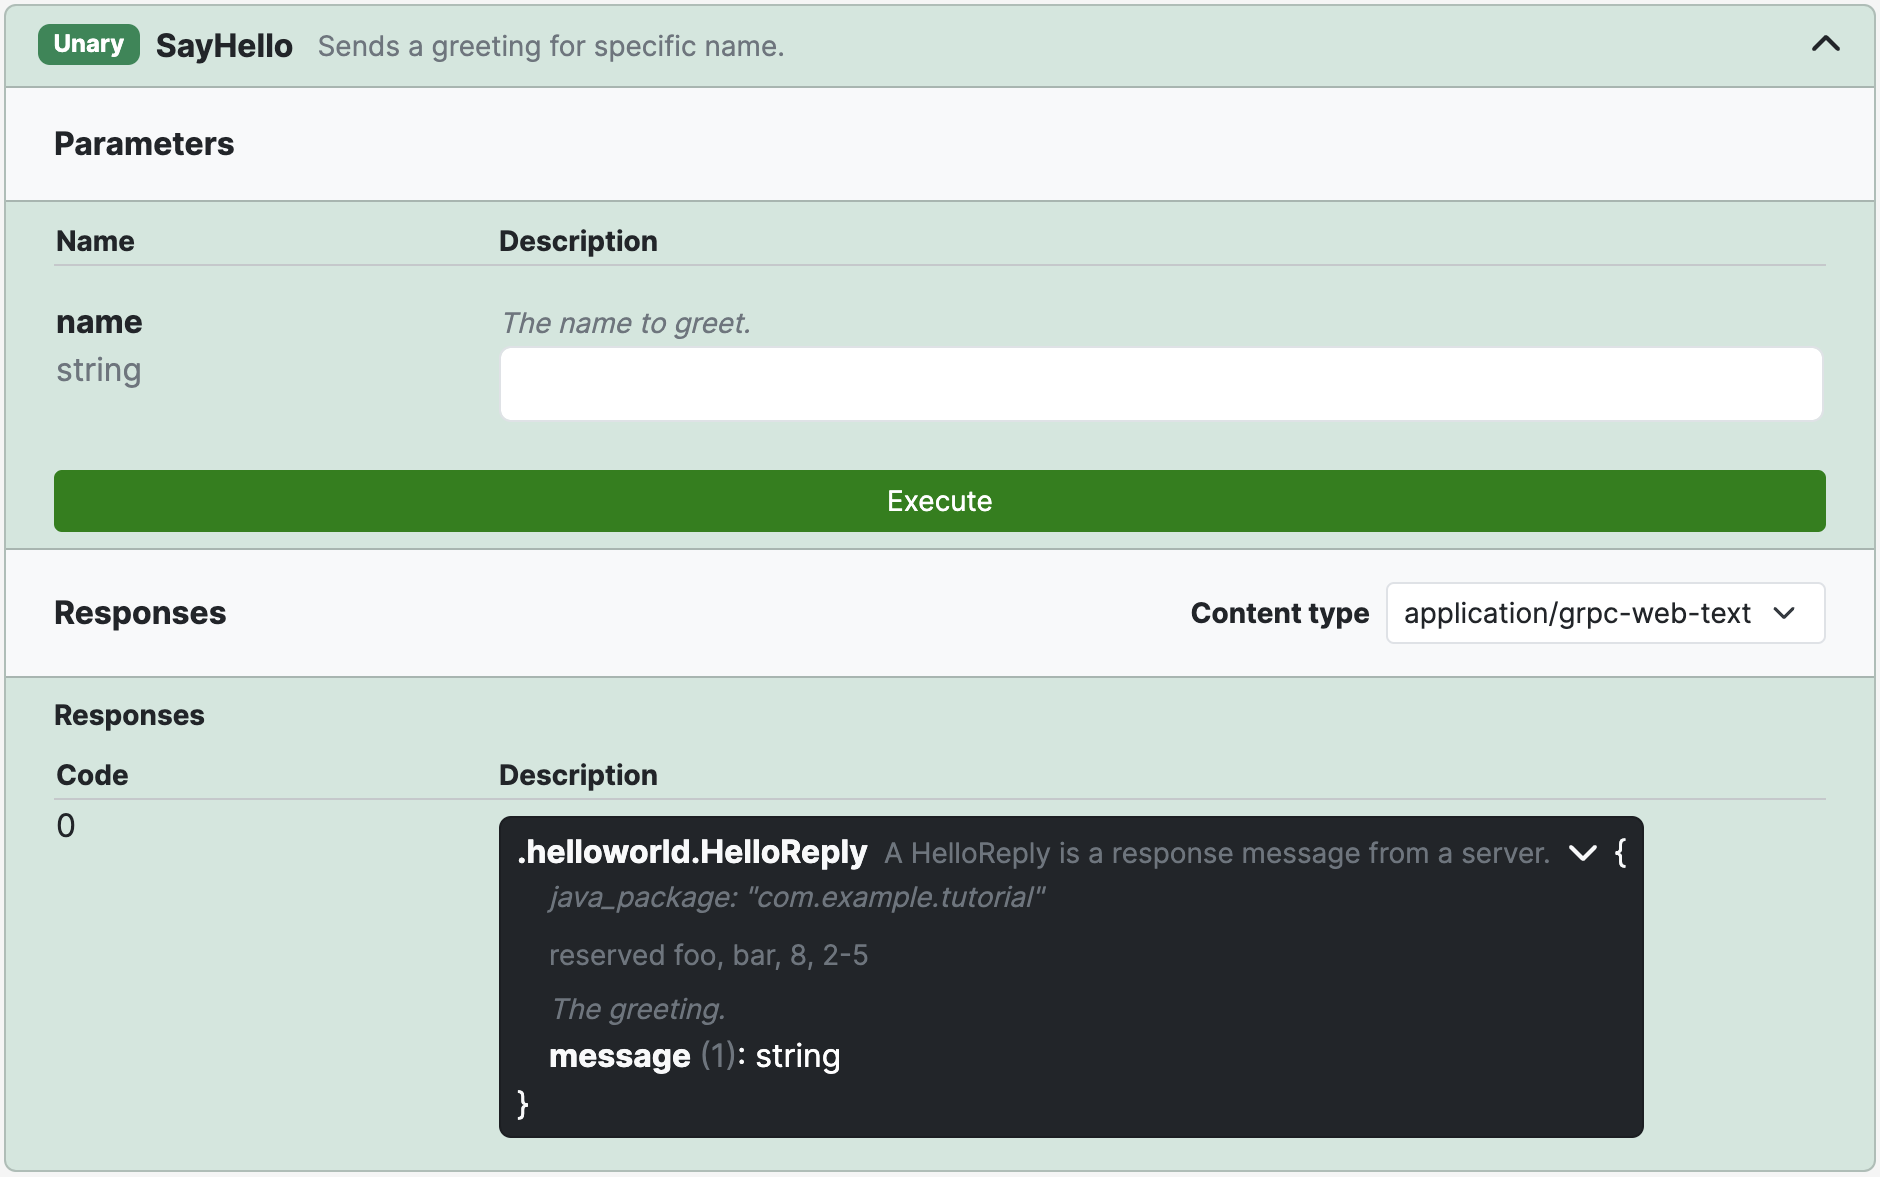
\includegraphics[width=0.8\textwidth]{images/implementation/screenshots/method}
    \caption{Method overview}
    \label{fig:implementation-screenshots-method}
\end{figure}

\begin{figure}[!htb]
    \centering
    \captionsetup{justification=centering}
    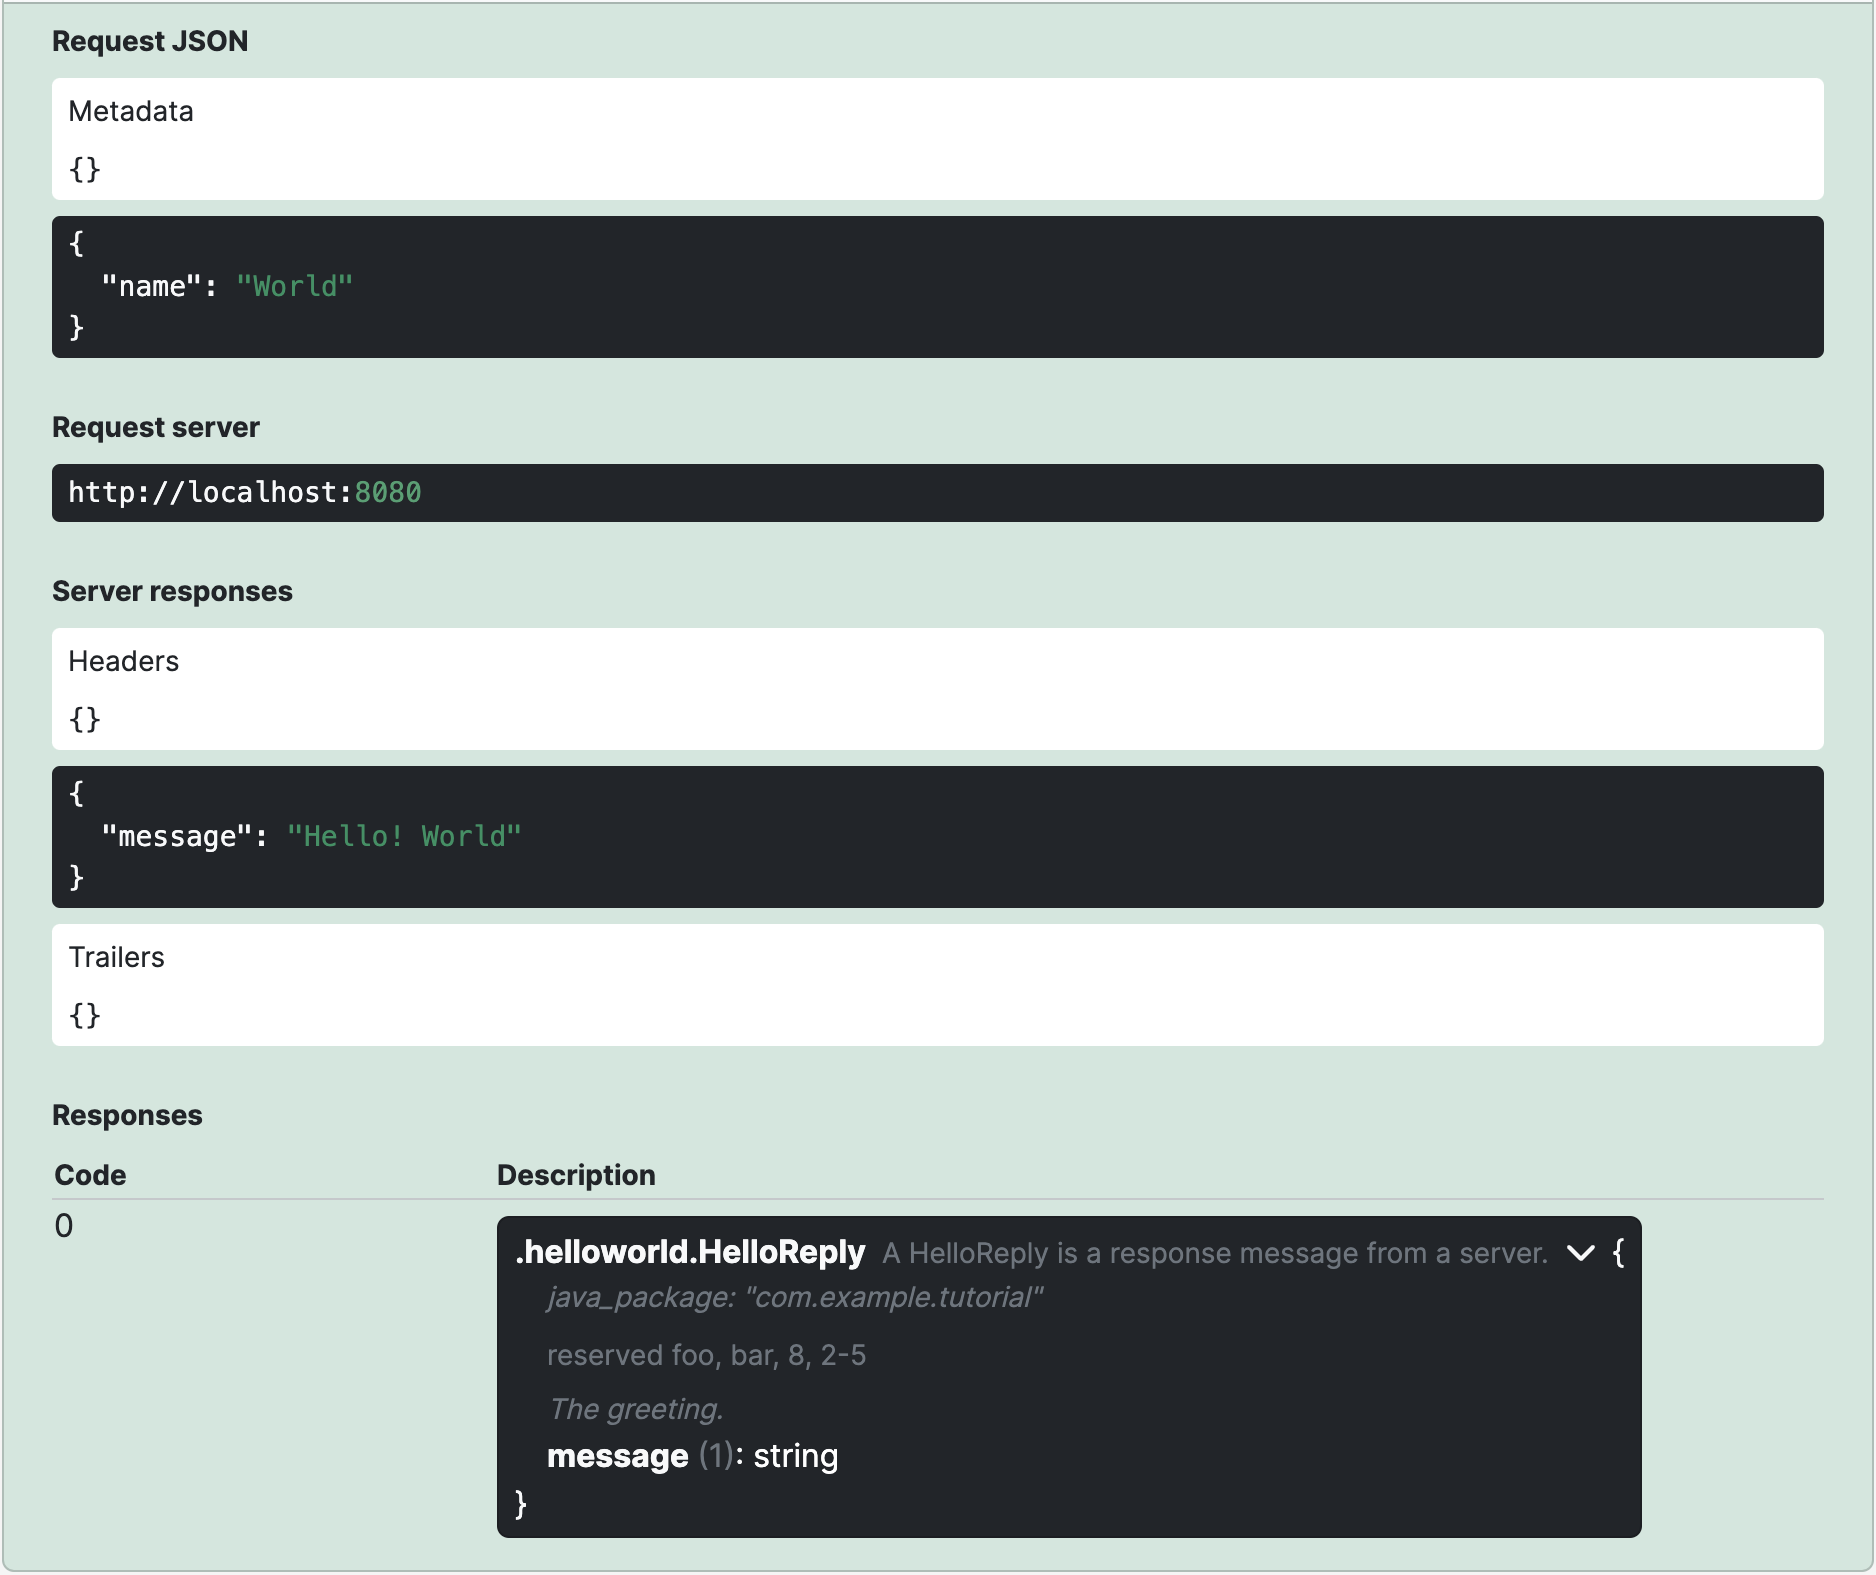
\includegraphics[width=0.8\textwidth]{images/implementation/screenshots/response}
    \caption{Method execution response}
    \label{fig:implementation-screenshots-response}
\end{figure}


\begin{figure}[!htb]
    \centering
    \captionsetup{justification=centering}
    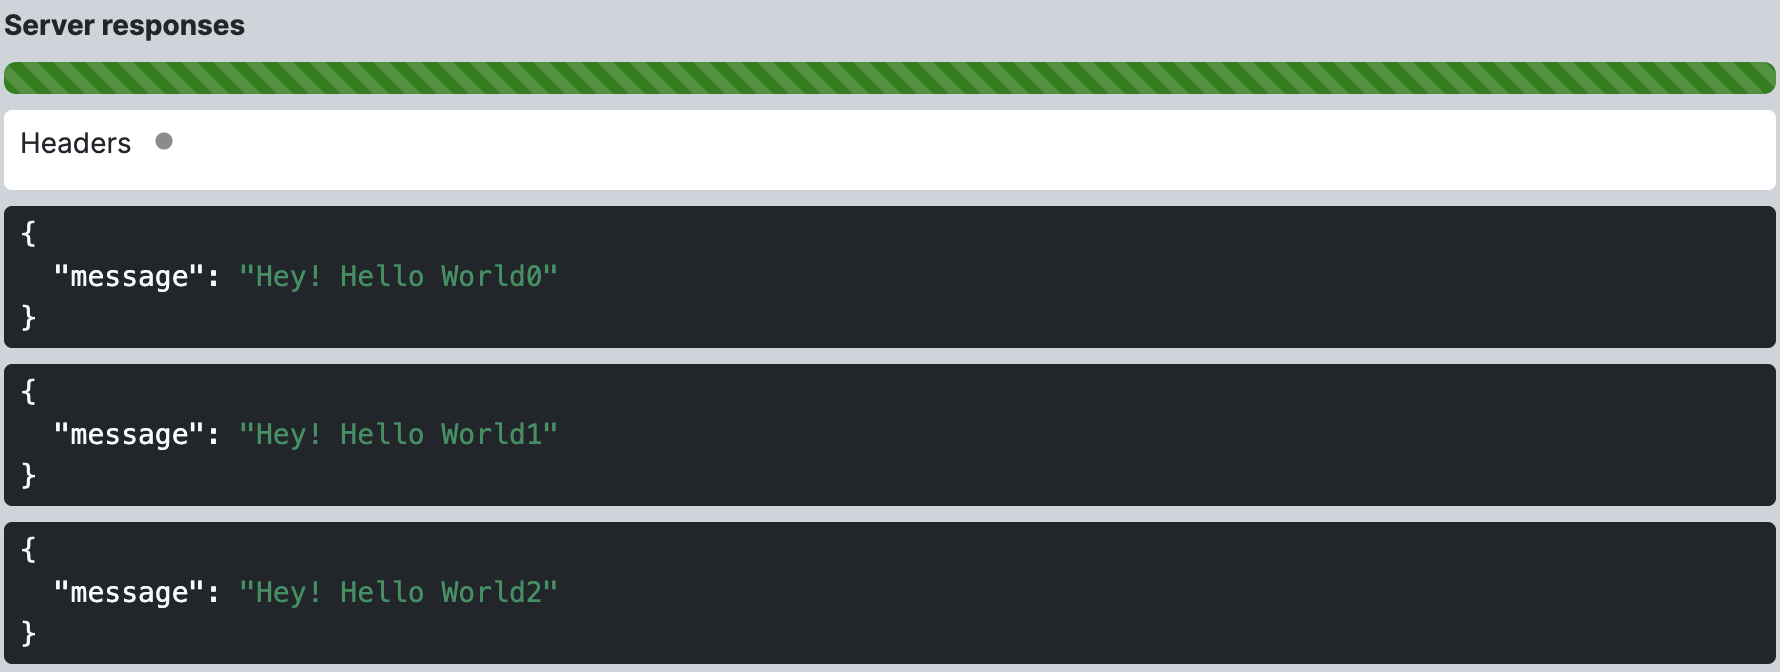
\includegraphics[width=0.8\textwidth]{images/implementation/screenshots/responses-streaming}
    \caption{Method execution response -- server streaming}
    \label{fig:implementation-screenshots-responses-streaming}
\end{figure}


\begin{figure}[!htb]
    \centering
    \captionsetup{justification=centering}
    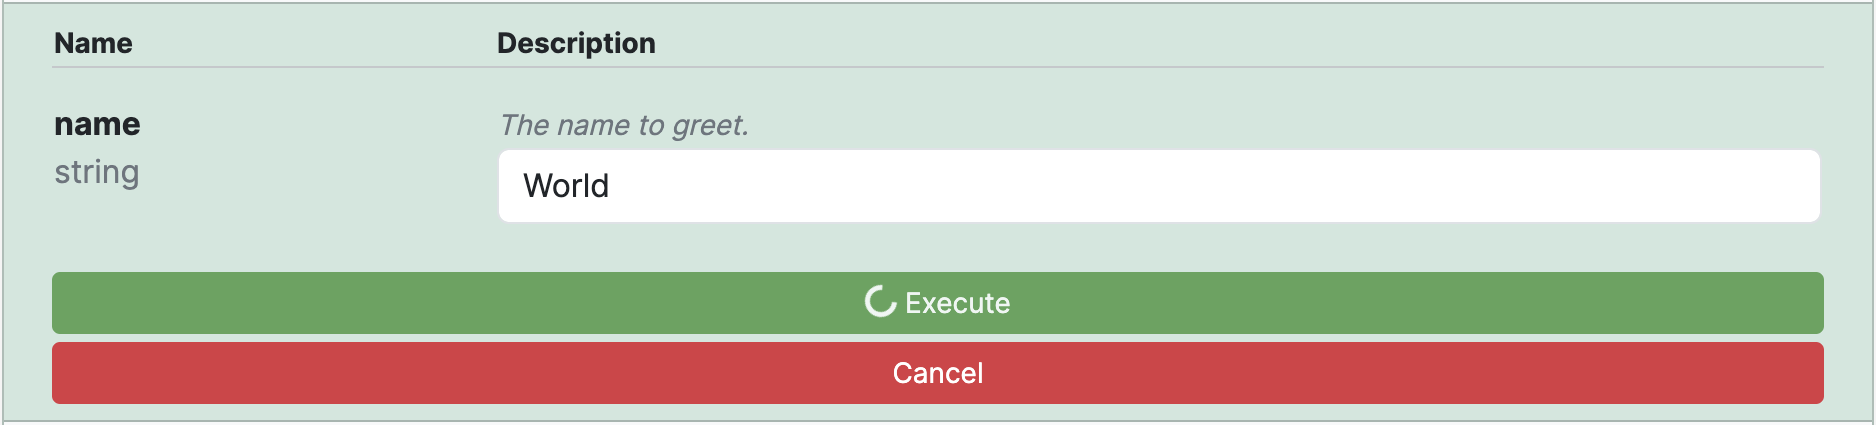
\includegraphics[width=0.75\textwidth]{images/implementation/screenshots/execution-pending}
    \caption{Method execution pending state}
    \label{fig:implementation-screenshots-execution-pending}
\end{figure}

\begin{figure}[!htb]
    \centering
    \captionsetup{justification=centering}
    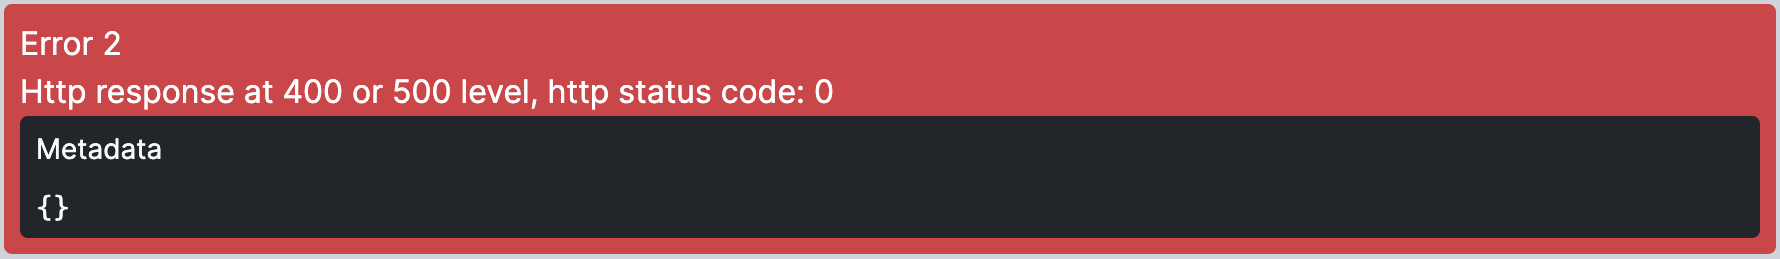
\includegraphics[width=0.75\textwidth]{images/implementation/screenshots/response-error}
    \caption{Method execution response error}
    \label{fig:implementation-screenshots-response-error}
\end{figure}

The input of a method is as a form.
Different input field types are shown in the figure~\ref{fig:implementation-screenshots-inputs}.
There is special handling for bytes input (file selection), strings, numbers, enums (dropdown selection), booleans (dropdown selection), oneof the fields grouping, and JSON input fields.
The JSON input fields are shown for repeated (arrays), maps, and messages fields.
Each JSON input contains also a tab with the JSON schema example and the interactive message type model (with expandable nested message types).
The same example and model also apply for the enum types, but the input is a dropdown selection (if it is not part of repeated).
Each field has a validation based on the schema definition.
The examples are shown in the figure~\ref{fig:implementation-screenshots-inputs-validation}.
The errors are shown after execution under the field with the error message and above the execution button.
The execution button is disabled until all fields are valid.

\begin{figure}[!htb]
    \centering
    \captionsetup{justification=centering}

    \begin{subfigure}{.33\textwidth}
        \centering
        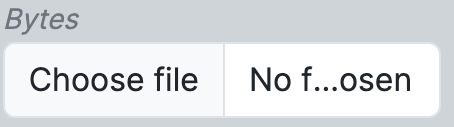
\includegraphics[width=.95\linewidth]{images/implementation/screenshots/input-bytes}
        \caption{Bytes}
    \end{subfigure}%
    \begin{subfigure}{.33\textwidth}
        \centering
        
\includegraphics[width=.95\linewidth]{images/implementation/screenshots/input-number}
        \caption{Number}
    \end{subfigure}
    \begin{subfigure}{.33\textwidth}
        \centering
        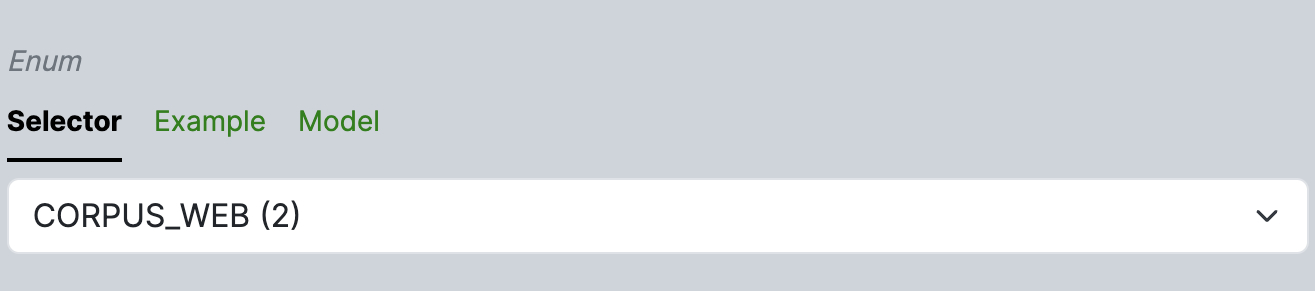
\includegraphics[width=.95\linewidth]{images/implementation/screenshots/input-enum}
        \caption{Enum}
    \end{subfigure}%

    \begin{subfigure}{.33\textwidth}
        \centering
        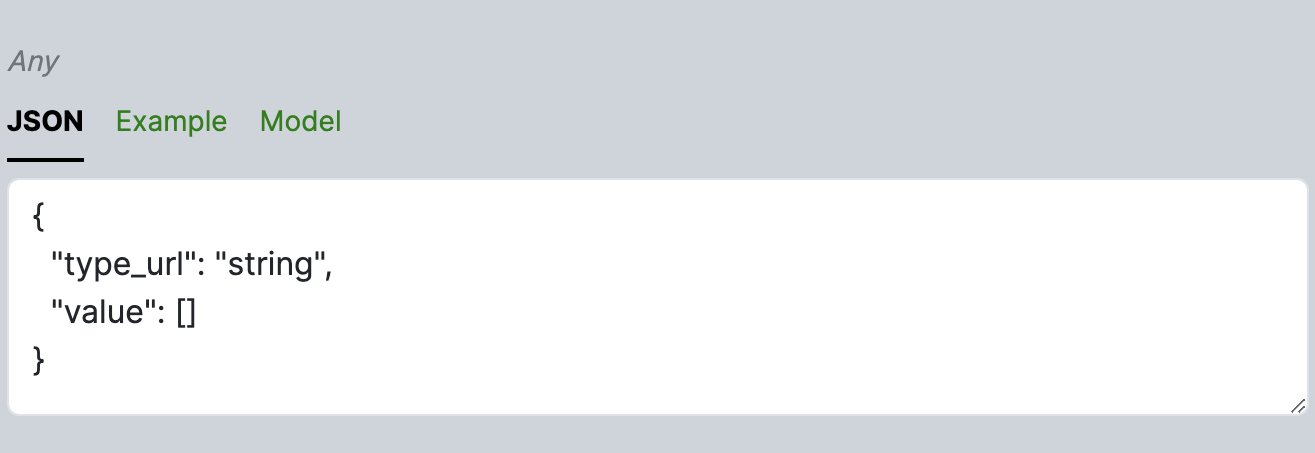
\includegraphics[width=.95\linewidth]{images/implementation/screenshots/input-json-field}
        \caption{JSON (message type, repeated, map)}
    \end{subfigure}
    \begin{subfigure}{.33\textwidth}
        \centering
        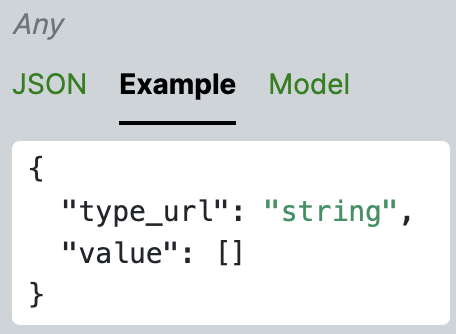
\includegraphics[width=.95\linewidth]{images/implementation/screenshots/input-json-example}
        \caption{JSON - example}
    \end{subfigure}%
    \begin{subfigure}{.33\textwidth}
        \centering
        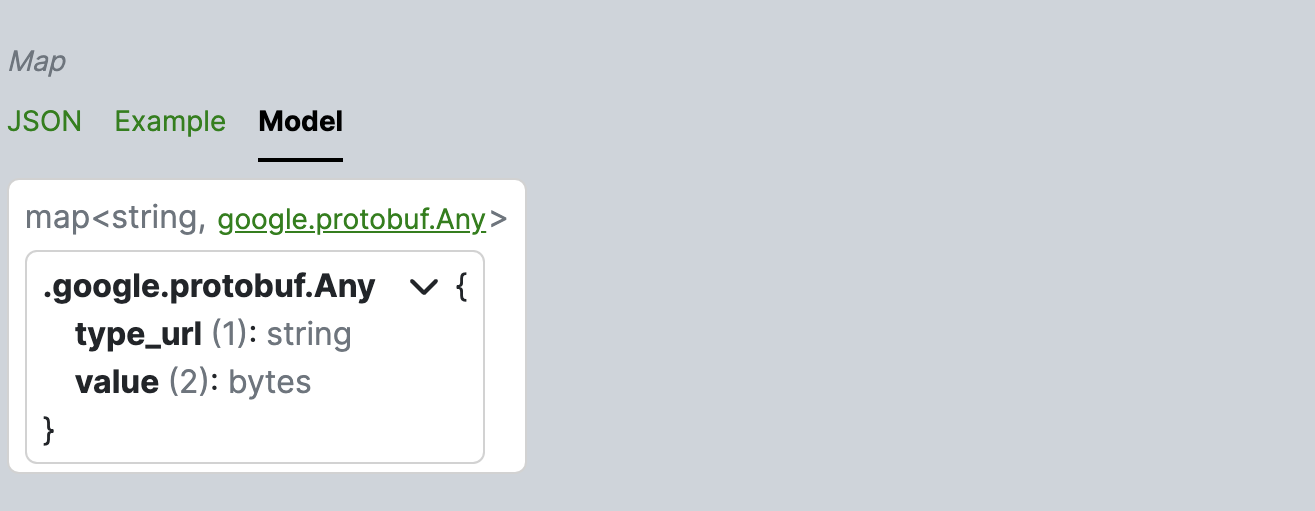
\includegraphics[width=.95\linewidth]{images/implementation/screenshots/input-map}
        \caption{Model}
    \end{subfigure}

    \begin{subfigure}{.33\textwidth}
        \centering
        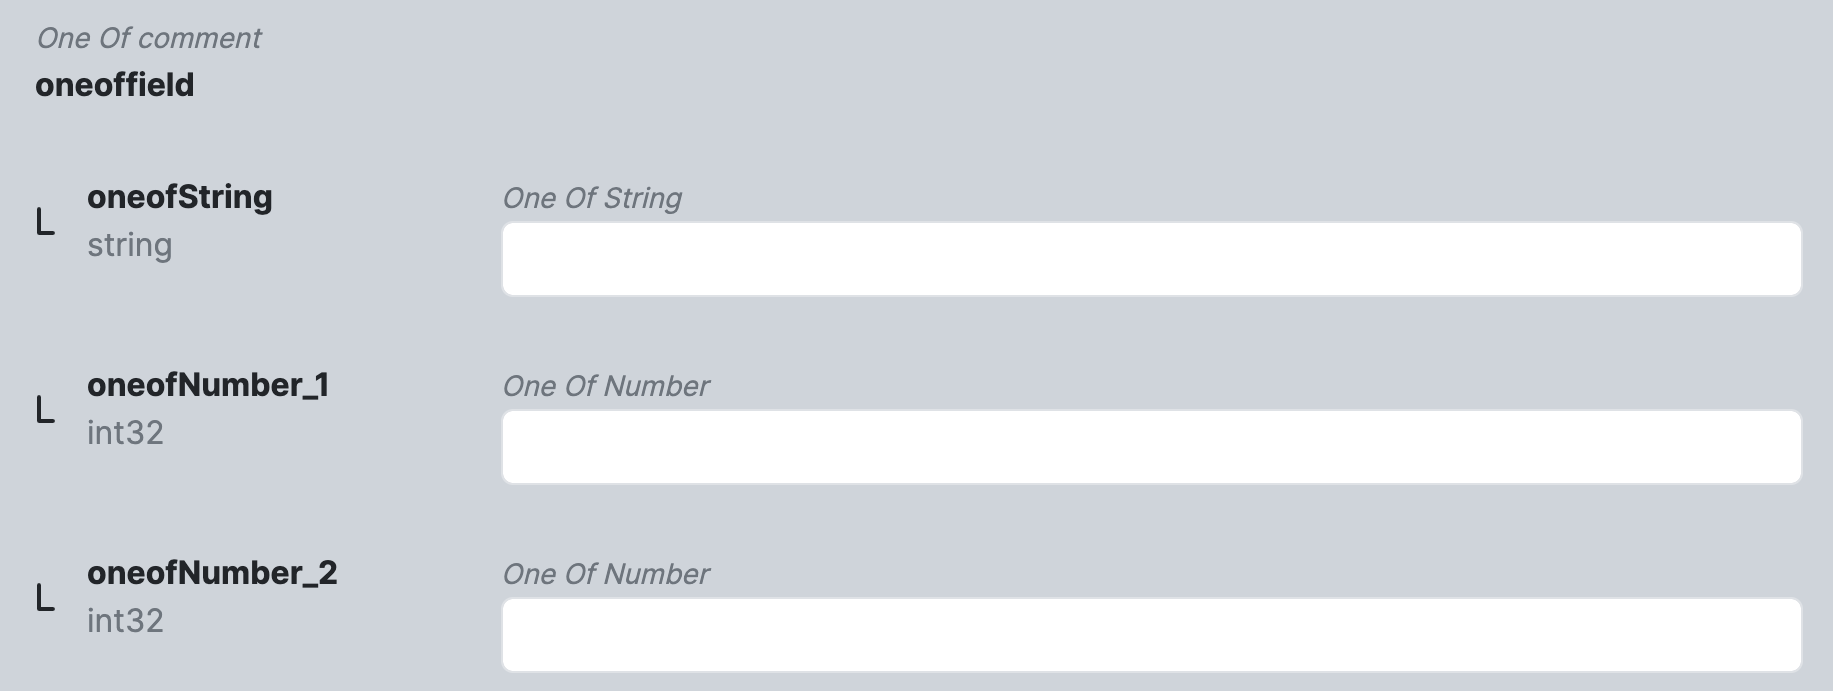
\includegraphics[width=.95\linewidth]{images/implementation/screenshots/input-oneof}
        \caption{Oneof}
    \end{subfigure}%
    \begin{subfigure}{.33\textwidth}
        \centering
        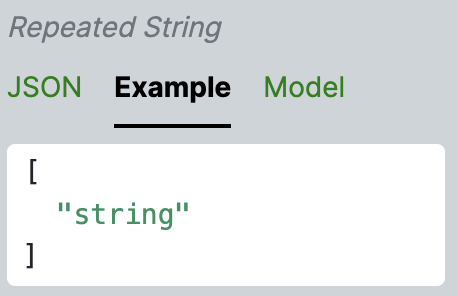
\includegraphics[width=.95\linewidth]{images/implementation/screenshots/input-repeated}
        \caption{Repeated - example}
    \end{subfigure}

    \caption{Method execution input fields}
    \label{fig:implementation-screenshots-inputs}
\end{figure}

\begin{figure}[!htb]
    \centering
    \captionsetup{justification=centering}

    \begin{subfigure}{1\textwidth}
        \centering
        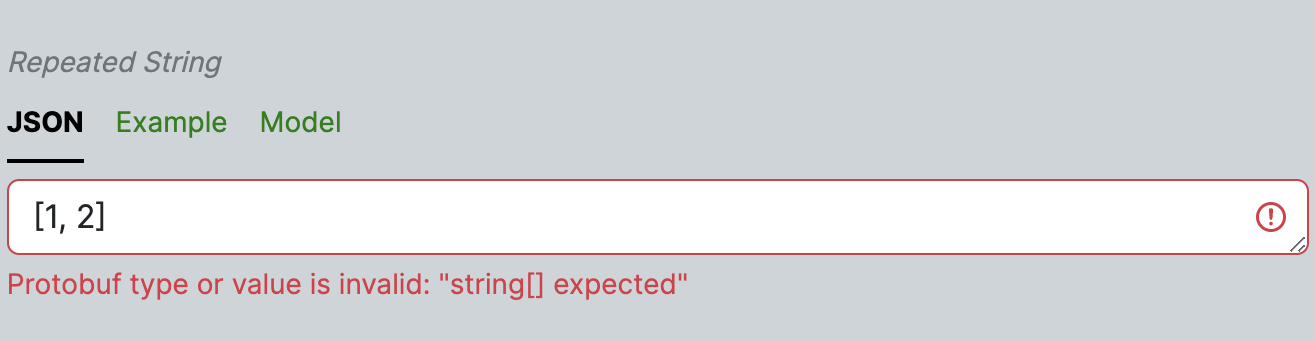
\includegraphics[width=.8\linewidth]{images/implementation/screenshots/input-validation-error}
        \caption{Field}

        \centering
        
\includegraphics[width=.8\linewidth]{images/implementation/screenshots/input-validation-error-button}
        \caption{Button}
    \end{subfigure}%

    \caption{Input validation}
    \label{fig:implementation-screenshots-inputs-validation}
\end{figure}


Message types are the next section on a website.
The expanded message type is shown in the figure~\ref{fig:implementation-screenshots-message-type}.
It shows the documentation comments and options for the message type itself, as well as for the fields.
All types of fields are shown, including repeated (as an array), maps, and oneof the fields.
Green text with underlining indicates an expandable message type.
The expanded message type is shown in the figure~\ref{fig:implementation-screenshots-message-type-field-expansion}.
If the expanded message type contains another nested message type, it is also expandable.
Each expansion rendering is done after clicking on the field, which prevents issues with recursive types.

\begin{figure}[!htb]
    \centering
    \captionsetup{justification=centering}

    \begin{subfigure}{.5\textwidth}
        \centering
        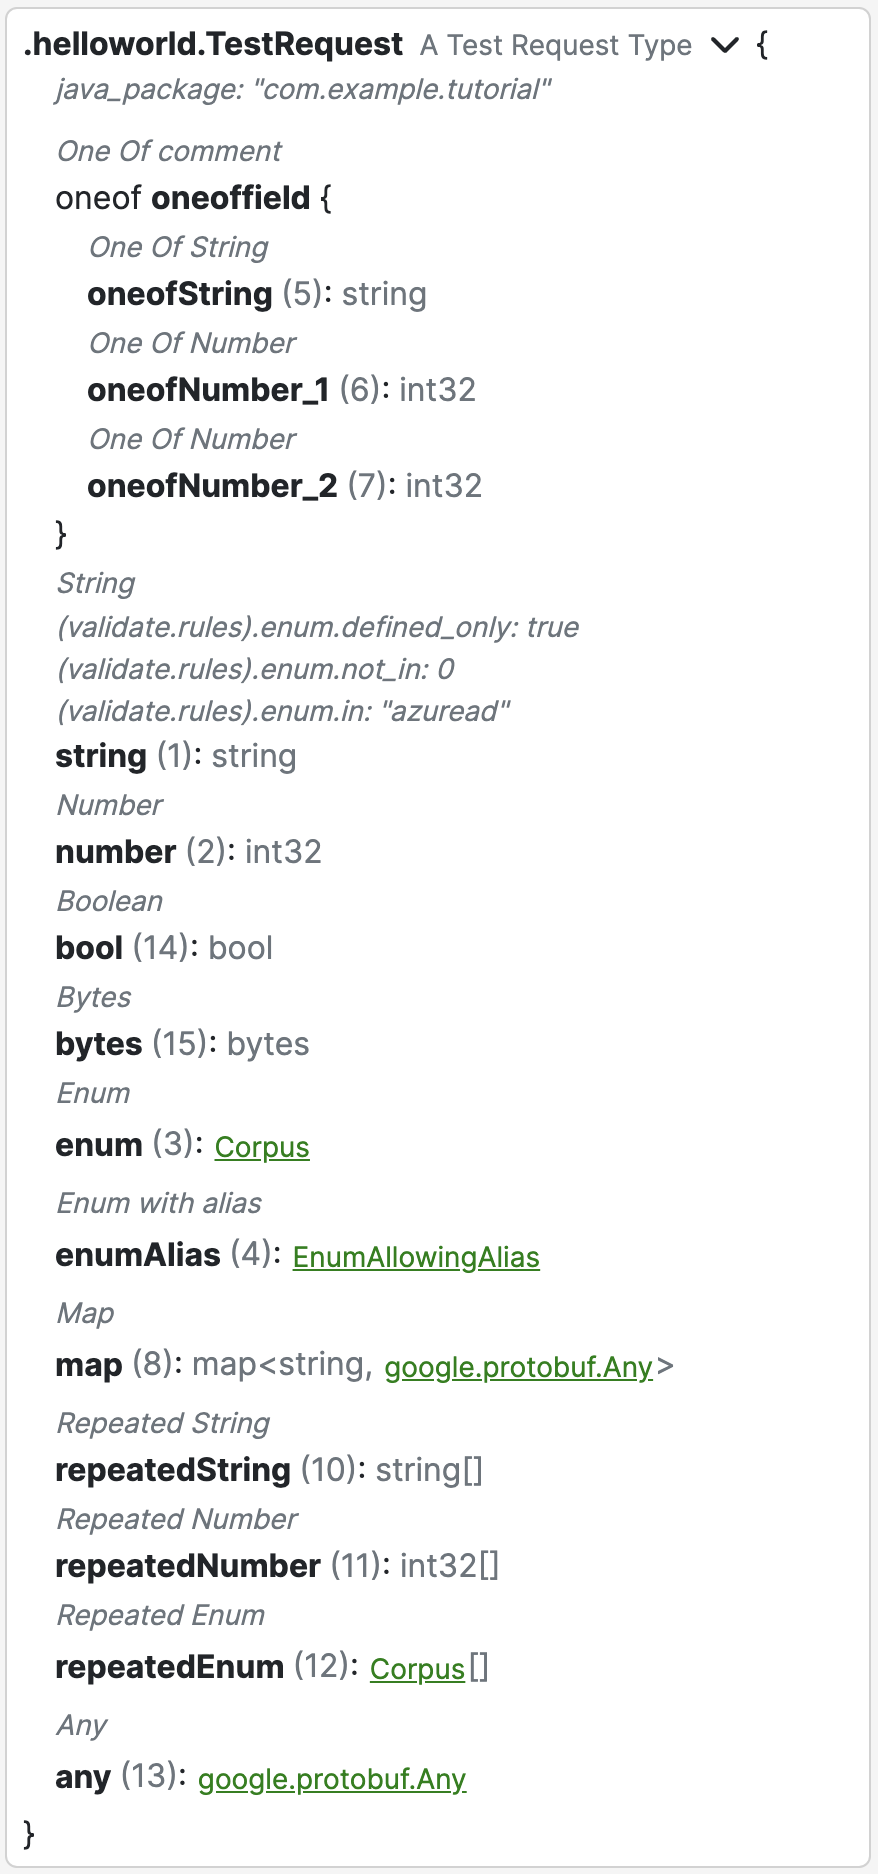
\includegraphics[width=.95\linewidth]{images/implementation/screenshots/message-type}
        \caption{Message type overview}
        \label{fig:implementation-screenshots-message-type}
    \end{subfigure}%
    \begin{subfigure}{.5\textwidth}
        \centering
        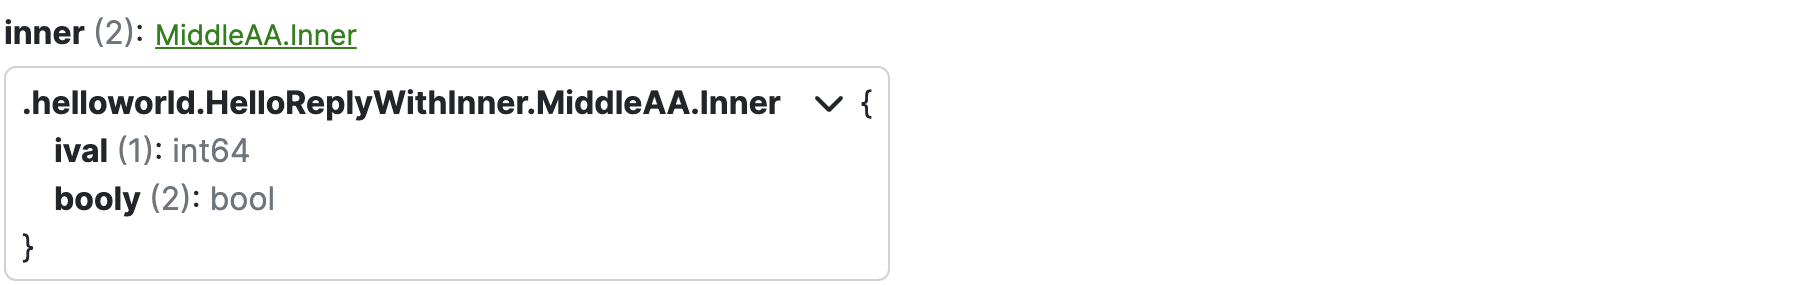
\includegraphics[width=.95\linewidth]{images/implementation/screenshots/message-type-field-expansion}
        \caption{Message type expanded}
        \label{fig:implementation-screenshots-message-type-field-expansion}

        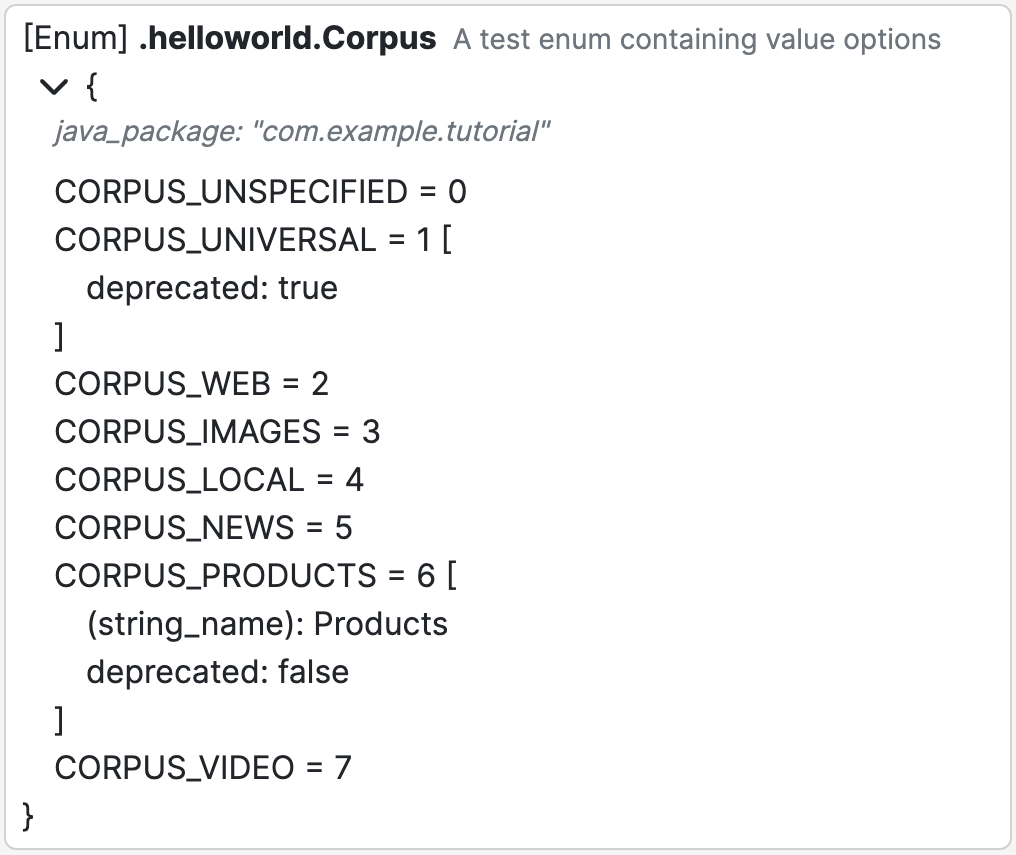
\includegraphics[width=0.95\linewidth]{images/implementation/screenshots/enum}
        \caption{Enum overview}
        \label{fig:implementation-screenshots-enum}
    \end{subfigure}%

    \caption{Message type and enum type}
\end{figure}

The website ends with enums.
The expanded enum is shown in the figure~\ref{fig:implementation-screenshots-enum}.
It shows the documentation comments and options for the enum itself, as well as for the values.
The values are shown as keys with their respective numbers.
The enum value options are shown in brackets after the value name, copying the protobuf syntax.

All the functionality and design allow the user to navigate through the proto file services, methods, message types, and enums and see the documentation comments.
When the user selects a method, they can execute it with the input form and see the response.
For streaming requests, the user can see the responses gradually.
They can see the error message for errors.
This way, the user can test the gRPC server without implementing any client and preview documentation.


\section{Licensing}
For the implementation, I have used libraries that use the following licenses:
\begin{itemize}
    \item MIT\footnote{\url{https://choosealicense.com/licenses/mit/}},
    \item BSD-3-Clause\footnote{\url{https://opensource.org/license/bsd-3-clause}},
    \item Apache 2.0\footnote{\url{https://choosealicense.com/licenses/apache-2.0/}},
    \item ISC\footnote{\url{https://www.isc.org/licenses/}},
    \item CC-BY-4.0\footnote{\url{https://creativecommons.org/licenses/by/4.0/}}.
\end{itemize}

The list of libraries and their licenses is captured in tables~\ref{tab:libraries-licenses} and~\ref{tab:libraries-licenses-dev}.
The rights and limitations of these licenses are then shown in table~\ref{tab:licenses}.

\begin{table}[hbt!]
    \centering
    \captionsetup{justification=centering}
    \begin{tabular}{|l|l|l|l|l|l|}
        \hline
        & \textbf{MIT} & \textbf{BSD-3-Clause} & \textbf{Apache 2.0} & \textbf{CC-BY-4.0} & \textbf{ISC} \\ \hline
        \textbf{Permissions}         &              &                       &                     &                    &              \\ \hline
        Commercial use               & \checkmark   & \checkmark            & \checkmark          & \checkmark         & \checkmark   \\ \hline
        Modification                 & \checkmark   & \checkmark            & \checkmark          & \checkmark         & \checkmark   \\ \hline
        Distribution                 & \checkmark   & \checkmark            & \checkmark          & \checkmark         & \checkmark   \\ \hline
        Patent use                   & -            & -                     & \checkmark          & x                  & -            \\ \hline
        Private use                  & \checkmark   & \checkmark            & \checkmark          & \checkmark         & \checkmark   \\ \hline
        &              &                       &                     &                    &              \\ \hline
        \textbf{Conditions}          &              &                       &                     &                    &              \\ \hline
        License and copyright notice & \checkmark   & \checkmark            & \checkmark          & \checkmark         & \checkmark   \\ \hline
        State changes                & -            & -                     & \checkmark          & \checkmark         & -            \\ \hline
        &              &                       &                     &                    &              \\ \hline
        \textbf{Limitations}         &              &                       &                     &                    &              \\ \hline
        Trademark use                & -            & -                     & x                   & x                  & -            \\ \hline
        Liability                    & x            & x                     & x                   & x                  & \checkmark   \\ \hline
        Warranty                     & x            & x                     & x                   & x                  & \checkmark   \\ \hline
    \end{tabular}
    \caption{Overview of licenses and their limitations}
    \label{tab:licenses}
\end{table}

All licenses allow private and commercial use, including distribution and possible modifications.
The only requirement is to
%keep the license and copyright notice and eventually
state changes if made (I have not made any changes to the libraries that require it).
% TODO Is it necessary to mention them somewhere in the project?
%All used libraries with their respective licenses can be found on the website


Because I have met the requirements of the licenses and their limitations, which allow me to use the libraries for free, I can use them for my work.

\newcommand{\library}[1]{%
    #1\tablefootnote{\url{https://www.npmjs.com/package/#1}}%
}

\newpage
\begin{table}[hbt!]
    \centering
    \captionsetup{justification=centering}
    \begin{tabular}{|l|l|l|}
        \hline
        \textbf{Library}                              & \textbf{License} \\ \hline
        \library{@fortawesome/fontawesome-svg-core}   & MIT              \\ \hline
        \library{@fortawesome/free-regular-svg-icons} & CC-BY-4.0, MIT   \\ \hline
        \library{@fortawesome/free-solid-svg-icons}   & CC-BY-4.0, MIT   \\ \hline
        \library{@fortawesome/react-fontawesome}      & MIT              \\ \hline
        \library{@hookform/resolvers}                 & MIT              \\ \hline
        \library{bootstrap}                           & MIT              \\ \hline
        \library{grpc-web}                            & Apache-2.0       \\ \hline
        \library{lodash}                              & MIT              \\ \hline
        \library{next}                                & MIT              \\ \hline
        \library{p-cancelable}                        & MIT              \\ \hline
        \library{protobufjs}                          & BSD-3-Clause     \\ \hline
        \library{protobufjs-cli}                      & BSD-3-Clause     \\ \hline
        \library{react}                               & MIT              \\ \hline
        \library{react-bootstrap}                     & MIT              \\ \hline
        \library{react-dom}                           & MIT              \\ \hline
        \library{react-hook-form}                     & MIT              \\ \hline
        \library{react-syntax-highlighter}            & MIT              \\ \hline
        \library{sass}                                & MIT              \\ \hline
        \library{yup}                                 & MIT              \\ \hline
    \end{tabular}
    \caption{List of libraries and their licenses}
    \label{tab:libraries-licenses}
\end{table}

\newpage
\begin{table}[hbt!]
    \centering
    \captionsetup{justification=centering}
    \begin{tabular}{|l|l|l|}
        \hline
        \textbf{Development Library}              & \textbf{License} \\ \hline
        \library{@testing-library/jest-dom}       & MIT              \\ \hline
        \library{@testing-library/react}          & MIT              \\ \hline
        \library{@types/jest}                     & MIT              \\ \hline
        \library{@types/lodash}                   & MIT              \\ \hline
        \library{@types/node}                     & MIT              \\ \hline
        \library{@types/react}                    & MIT              \\ \hline
        \library{@types/react-dom}                & MIT              \\ \hline
        \library{@types/react-syntax-highlighter} & MIT              \\ \hline
        \library{cross-env}                       & MIT              \\ \hline
        \library{eslint}                          & MIT              \\ \hline
        \library{eslint-config-next}              & MIT              \\ \hline
        \library{eslint-config-prettier}          & MIT              \\ \hline
        \library{jest}                            & MIT              \\ \hline
        \library{jest-environment-jsdom}          & MIT              \\ \hline
        \library{prettier}                        & MIT              \\ \hline
        \library{typescript}                      & Apache-2.0       \\ \hline
        \library{lerna}                           & MIT              \\ \hline
        \library{rimraf}                          & ISC              \\ \hline
    \end{tabular}
    \caption{List of development libraries and their licenses}
    \label{tab:libraries-licenses-dev}
\end{table}